\documentclass{beamer}

\mode<presentation> {
	\usetheme{Madrid}
}

\usepackage[utf8]{inputenc}
\usepackage{graphicx}
\usepackage{amsmath}
\usepackage{hyperref}
\usepackage{siunitx}
\usepackage{enumitem}

\setbeamertemplate{caption}{\insertcaption\par}
\setbeamerfont{caption}{size=\scriptsize}

\newcommand{\includepic}[3]{
	\parbox{0.65\textwidth}{
	#1}\hspace{0.04\textwidth}
	\parbox{0.25\textwidth}{
	\begin{figure}
		\includegraphics[width=0.25\textwidth]{#2}
		\caption{#3}
	\end{figure}
	}
}
\newcommand\laplace{\mathop{}\!\mathbin\bigtriangleup}
\newcommand*{\boxedcolor}{red}
\renewcommand{\boxed}[1]{\textcolor{\boxedcolor}{%
  \fbox{\normalcolor$\displaystyle#1$}}}
	

\title[TMA4220 - Project]{How to bake the perfect cake}
\author[Simon, Hans]{Simon Thomä, Hans Pieper}
\institute[]{
	Numerical Solution of Partial Differential Equations Using Element Methods
}

\date{\today}

\begin{document}

	\begin{frame}
		\titlepage
	\end{frame}
	
	\begin{frame}
		\frametitle{Overview}
		\tableofcontents
	\end{frame}

% !TeX spellcheck = en_GB 

\section{\label{sec::problem}Problem}
The theoretical problem we want to solve is the heat equation, which is given by:
\begin{align}
	\frac{\partial u}{\partial t} &= \nabla(\alpha\nabla u) \label{eqn::strongForm}\\
	u(\vec{x},t)|_{\partial\Omega^D} &= u^D \label{eqn::dirichlet}\\
	\left.\left( \frac{\partial u(\vec{x},t)}{\partial \nu}\right)\right|_{\partial\Omega^N} &= g \label{eqn::neumann}\\
	u(\vec{x},t)|_{t=0} &=u_0(\vec{x}) \label{eqn::u_0}
\end{align}
Where:
\begin{itemize}
	\item $u(\vec{x},t)$ is the heat function.
	\item $\alpha$ is a constant denoting the thermal diffusivity.
	\item $\Omega$ is the domain of the problem.
	\item $\partial\Omega^D$ is the part of the boundary with Dirichlet conditions.
	\item $\partial\Omega^N$ is the part of the boundary with Neumann conditions.
	\item $\nu$ is the normal vector on the boundary.
\end{itemize} 
% !TeX spellcheck = en_GB 

\section{\label{sec::setupSystem}Setting up the System}
In this section we find a relaxation of the problem stated in section \ref{sec::problem}. Multiplying both sides of (\ref{eqn::strongForm}) with an arbitrary test function $v\in V:=H^1(\Omega)$ and integrating over the domain, we get the weak formulation:
\begin{equation*}
        \int\limits_{\Omega} \frac{\partial u}{\partial t} v = \int\limits_{\Omega} (\nabla(\alpha\nabla u)) v.
\end{equation*}
Integrating the right hand side by parts will result in:
\begin{equation*}
        \int\limits_{\Omega} \frac{\partial u}{\partial t} v = -\int\limits_{\Omega} \alpha(\nabla u) \cdot (\nabla v) + \int\limits_{\partial \Omega} \alpha v (\nabla u) \cdot \nu.
\end{equation*}
Using
\begin{equation*}
        (\nabla u)\cdot \nu = \frac{\partial u}{\partial \nu} = g
\end{equation*}
from (\ref{eqn::neumann}) leads to:
\begin{equation}
        \label{eqn::weakForm}
        \int\limits_{\Omega} \frac{\partial u}{\partial t} v = -\int\limits_{\Omega} \alpha(\nabla u) \cdot (\nabla v) +  \int\limits_{\partial\Omega^N} \alpha gv + \int\limits_{\partial \Omega^D} \alpha v (\nabla u) \cdot \nu.
\end{equation}
Using the above we can now define the bilinear form $a$ and linear operator $L$:
\begin{equation}
        a(u,v)=\int\limits_{\Omega} \left(\frac{\partial u}{\partial t} v +  \alpha(\nabla u) \cdot (\nabla v) \right) \\
        L(v) = \int\limits_{\partial\Omega^N} \alpha gv.
\end{equation}
From now on we assume that $a$ is bounded and coerzive and that $L$ is bounded. This will assure that we can use Cea's Lemma \cite{quarteroni2009numerical} and that thereby the heat equation has a unique solution.

To solve the weak formulation (\ref{eqn::weakForm}) numerically we discretise our domain $\Omega$. Our notation will follow \cite{quarteroni2009numerical}. Also we will not state every step in detail, if you wish, to get deeper insights in the theory behind it, we also recommend reading \cite{quarteroni2009numerical}.

Let $\mathcal{T}_h$ be a set of non overlapping tetrahedrons covering $\Omega$ and $\mathcal{N}={N_1,\dots N_{n_h}}$ the nodes of this mesh. As the theory about this is not new, and not closely related, to our problem, we don't want to go into detail about this. The approximated domain is then $\Omega_h:=\bigcup_{K\in\mathcal{T}_h}K$.

As an approximation of the functions in $V$, we use the Galerkin method, searching only for functions in $X_h:=\{v_h\in C^0(\overline{\Omega}_h) : v_h|_K \text{ linear } \forall K\in \mathcal{T}_h\}\subset V$. These are the continuous functions on $\Omega_h$, that are piecewise linear on each tetrahedron.

A basis for this space is given by the characteristic Lagrangian functions $\phi_j\in\ X_h, j=1,\dots n_h$, with $\phi_j(N_i) = \delta_{ij}$. So we can write every $v_h\in X_h$ in the following way:
\begin{equation*}
        v_h(x) = \sum_{j=1}^{j=n_h}v_j\phi_j.
\end{equation*}

On this space the equation (\ref{eqn::weakForm}) is equivalent to the following:
\begin{equation}
\label{eqn::discreticedWeakForm}
\begin{aligned}
        \int\limits_{\Omega} \sum_i \frac{\partial u_i}{\partial t} \phi_i \phi_j = &-\int\limits_{\Omega} \sum_i \alpha u_i(\nabla \phi_i) \cdot (\nabla \phi_j) \\
        &+ \int\limits_{\partial\Omega^N} \alpha g\phi_j \\
        &+ \int\limits_{\partial\Omega^D} \sum_i \alpha u_i (\nabla \phi_i) \cdot \nu \phi_j & \forall j.
\end{aligned}
\end{equation}

Considering the case of homogeneous Dirichlet conditions (i.e. $u^D=0$), we only have to search on the subspace $V_h:=\mathring{X}_h:=\{v_h\in X_h : v_h|_{\partial\Omega_h^D} = 0\}$. Let WLOG be the last indices $n_D,\dots n_h$, the indices of the nodes on the Dirichlet boundary. As $v_h\in V_h$ leads to $v_j = 0, \forall j\geq n_D$, (\ref{eqn::discreticedWeakForm}) becomes:
\begin{equation}
\label{eqn::homogeneousForm}
\begin{aligned}
        \int\limits_{\Omega} \sum_i \frac{\partial u_i}{\partial t} \phi_i \phi_j = &-\int\limits_{\Omega} \sum_i \alpha u_i(\nabla \phi_i) \cdot (\nabla \phi_j) \\
        &+ \int\limits_{\partial\Omega^N} \alpha g\phi_j
         & \forall j < n_D.
\end{aligned}
\end{equation}

We can reduce the non-homogeneous case to the homogeneous one, by introducing a lifting $R_g\in X_h$ as follows:
\begin{equation*}
        R_g(x) := \sum_{i=n_D}^{n_h}d_i \phi_i(x),
\end{equation*}
where $d_i:=u^D(N_i)$. With the homogeneous solution
\begin{equation*}
        \mathring{u} := \sum_{i=1}^{n_D-1}u_i \phi_i(x),
\end{equation*}
the final solution is given by
\begin{equation}
        \label{eqn::fullu}
        u = \mathring{u} + R_g.
\end{equation}


To find this homogeneous solution, we insert (\ref{eqn::fullu}) in (\ref{eqn::homogeneousForm}) and get:
\begin{equation}
\label{eqn::finalDiscreticedForm}
\begin{aligned}
        \int\limits_{\Omega} \sum_{i=1}^{n_D-1} \frac{\partial u_i}{\partial t} \phi_i \phi_j = &-\int\limits_{\Omega} \sum_{i=1}^{n_D-1} \alpha u_i(\nabla \phi_i) \cdot (\nabla \phi_j) \\
        &+ \int\limits_{\partial\Omega^N} \alpha g\phi_j \\
        &-        \int\limits_{\Omega} \sum_{i=n_D}^{n_h}\left( \dot{d}_i \phi_i \phi_j  + \alpha d_i(\nabla \phi_i) \cdot (\nabla \phi_j)\right)
         & \forall j,
\end{aligned}
\end{equation}
with $\dot{d}_i:=\frac{\partial u^D}{\partial t}(N_i)$.

We now define the matrices $M$, $A$ and the vectors $N$, $D$ by:
\begin{align*}
        M_{ij} &:=\int\limits_{\Omega} \phi_i \phi_j \\
        A_{ij} &:=\int\limits_{\Omega} \alpha (\nabla \phi_i) \cdot (\nabla \phi_j) \\
        N_{j} &:=\int\limits_{\partial\Omega^N} \alpha g\phi_j \\
        D_{j} &:=\int\limits_{\Omega} \sum_{k=n_D}^{n_h}\left( \dot{d}_k \phi_k \phi_j  + \alpha d_k(\nabla \phi_k) \cdot (\nabla \phi_j)\right),
\end{align*}
where $i,j=1,\dots (n_D-1)$. Using these we get the system of ordinary differential equations:
\begin{equation}
        \label{eqn::matrixForm}
        M\frac{\partial u}{\partial t} = -A u + N - D.
\end{equation}
How we solve these will be considered in the following section.

For the practical part we implemented functions, which can calculate these matrices and vectors. To do so we use the transformation properties of the barycentric coordinates from the basic element (triangle or higher dimensional equivalent). As we wanted to be able to solve the problem as general as possible, we allow $g$ and $d$ to be space and time dependent. If one of them depends on time, the corresponding vectors has to be calculated every time step in the solving progress of the differential equation (section \ref{sec::odesolver}). The thermal diffusivity $\alpha$ can differ between the elements, but we assume it to be constant within each.

% !TeX spellcheck = en_GB 

\section{\label{sec::odesolver}Solving the ODE}

From equation \ref{eqn::matrixForm} we get a system of $n_D-1$ ordinary differential equation of order 1, where at most the inhomogenious part can be non-linear. So we have to solve an initial value problem (IVP) of the form
\begin{flalign*}
	M\dot{u}=Au+v(t)
\end{flalign*}
on the interval $t\in\left[t_0,t_{max}\right]$ with initial value $u_0=u(t_0)$. The ODE can of course also be written as 
\begin{flalign*}
	\dot{u}=M^{-1}(Au+v(t))
\end{flalign*}
but inverting a matrix of size $(n_D-1)\times(n_D-1)$ would take probably at least $\mathcal{O}(n_D^3)$ \cite{li2009fastsolver} operations so is something that wants to be avoided, since e.g. in our case this would be of order $>10^{12}$. \\
To solve the IVP we implemented the following four different solvers. All of them are one step solvers, meaning to compute the next time step only the timestep before is used. Two of the solvers are explicit and two implicit. The advantage of an explicit solver is normaly, that for each time step only one matrix multiplication and one vector addition would be needed. Since in our case we have to solve for $M$ at all, this will not realy help. Also explicit methods are not stable especially over a long time \cite{damenreusken2006bible}. But baking a cake takes normaly more then 1 hour or 3600 seconds. The disadvantage of implicit methods is, that you have to invert a matrix every time step, therefor they are satble also over a long time. Finaly the methods we implemented and their iterations are
\begin{itemize}
	\item Implicit methods
	\begin{enumerate}[label=\arabic*.)]
		\item Forward Euler
		\begin{flalign*}
			u_{n+1}=u_n+hM^{-1}(Au_n+v(t_n))
		\end{flalign*}
		\item Improved Forward Euler
		\begin{flalign*}
			u_{n+1}=u_n+\frac{h}{2}M^{-1}\left(2Au_n+v(t_n)+v(t_{n+1})+hA\cdot M^{-1}\left(Au_n+v(t_n)\right)\right)
		\end{flalign*}
	\end{enumerate}
	\item Explicit methods
	\begin{enumerate}[resume,label=\arabic*.)]
		\item Backwards Euler
		\begin{flalign*}
			(M-hA)u_{n+1}=Mu_n+hv(t_n)
		\end{flalign*}
		\item Crank-Nicholson
		\begin{flalign*}
			(M-\frac{h}{2}A)u_{n+1}=(M+\frac{h}{2}A)u_n+\frac{h}{2}(v(t_n)+v(t_{n+1}))
		\end{flalign*}
	\end{enumerate}
\end{itemize}
So we have to solve a linear system in each time step for each of these methods. Instead of completly solving the system we want to do some steps of an iterative solver. The most convincing solver we found is the preconditioned conjugete gradient (PCG) method. This method is even implemented in MATLAB and can called with \emph{pcg}. As preconditioner we chose modified incomplete cholesky decomposition, which is also implemented and can be called by \emph{ichol}. The advantage of this combination is, that in case the matrix that has to be inverted is symmetric positiv definit (spd), also the preconditioning matrix for conjugate gradient is spd.

\begin{lstlisting}[language=bash]
\end{lstlisting}

For this we implemented


\section{\label{sec::modelling}Modelling the cake}
To model the baking process, we now only need a few more ingredients. First we have to know the thermal properties of cake dough and the baking form, which we will consider to be out of aluminium. For the dough \cite{baik1999modeling} found out, that the thermal diffusivity of cupcake dough, which should be close enough to our cake dough is $\alpha_{cake}=1.02\times 10^{-7} \SI{}{\meter/\second^2 } \text{ to } 1.698\times 10^{-7} \SI{}{\meter/\second^2}$. In the appendix of \cite{kothandaraman2006fundamentals} we find $\alpha_{Al} = 9.444\times 10^{-5} \SI{}{\meter/\second^2}$ for the thermal diffusivity of aluminium.

Second we need the mesh, which models the cake and the baking form. This is given on the course-webpage and can be seen in figure \ref{fig::mesh}, where the yellow part identifies an aluminium stick. The rod helps to heat up the cake from the inside. For the radius we choose $15\SI{}{\centi\meter}$, as we want to have a big cake, which has a realistic chance, to get baked in a reasonable time.

\begin{figure}[htp]
        \centering
        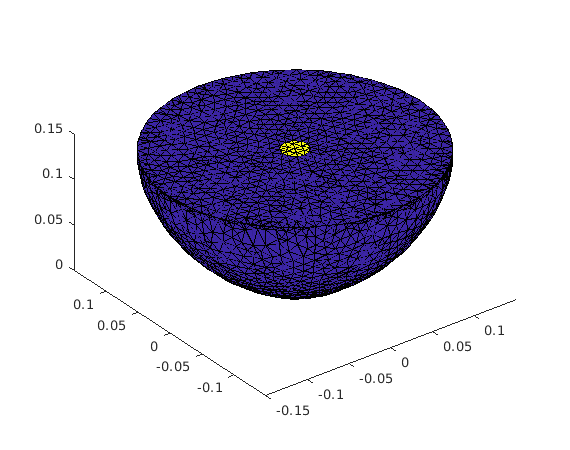
\includegraphics[width=0.5\textwidth]{figures/mesh.png}
        \caption{\label{fig::mesh} Mesh of the cake}
\end{figure}

% !TeX spellcheck = en_GB 

\section{\label{sec::results}Results}


	
	\begin{frame}
		\begin{center}
			\Large Questions?
		\end{center}
	\end{frame}

\end{document}
